\documentclass[UTF8,11pt,oneside]{ctexart}

\def\articletitle{大同订婚强奸案,怎么判对你最有利}
\usepackage{CJKfntef}
\usepackage{float}

\usepackage{geometry}
\geometry{a4paper,left=2cm,right=2cm,top=2cm,bottom=1cm}

\usepackage{graphicx}

\usepackage{hyperref}
\hypersetup{colorlinks=true, linkcolor=red}

\linespread{1.6}

\usepackage{fancyhdr}
\usepackage{ifthen}
\pagestyle{fancy}
\fancyhf{}
\setlength{\headheight}{14pt}
\fancyhead[R]{\ifthenelse{\value{page}>1}{\thepage}{}}
\fancyhead[C]{\ifthenelse{\value{page}>1}{\articletitle}{}}
\renewcommand\headrulewidth{0pt}

\usepackage{tcolorbox}
\tcbuselibrary{skins}

\newcommand{\zd}[1]{\textbf{\textcolor[RGB]{123,12,0}{#1}}} % 重点

\newcommand{\yinyong}[1]{% 引用
    \begin{tcolorbox}[enhanced,
        frame hidden, interior hidden,
        before skip = 5mm, left skip=10mm,
        borderline west={5pt}{0pt}{gray!50}]
        #1
    \end{tcolorbox}
}

\newcommand{\xhx}[1]{%下划线(模拟微信中的划线功能,用于标注我个人认为的文章中精彩的地方)
    \CJKunderline*[thickness=1.5pt, format=\color[RGB]{84,216,140}]{#1}
}

\newcommand{\biaoti}[1]{% 标题
    \section*{#1}
}

\newcommand{\SetSectionType} {
    \ctexset{
        section={
            number = \chinese{section},
            aftername={、},
            format=\Large\bfseries,
        }
    }
}



\begin{document}

\begin{center}
    \LARGE{\articletitle\footnotemark}
\end{center}
\footnotetext{
    原文出自公众号“远方青木”的文章 《\href{https://mp.weixin.qq.com/s/jbQR2PUOCrTViYaxCgKjjw}{\articletitle}》
}

拖延两年多的大同订婚强奸案出二审结果了。

驳回上诉,维持原判,判男方强奸罪成立,处3年有期徒刑,同时其母遭训诫。

\begin{figure}[H]
    \centering
    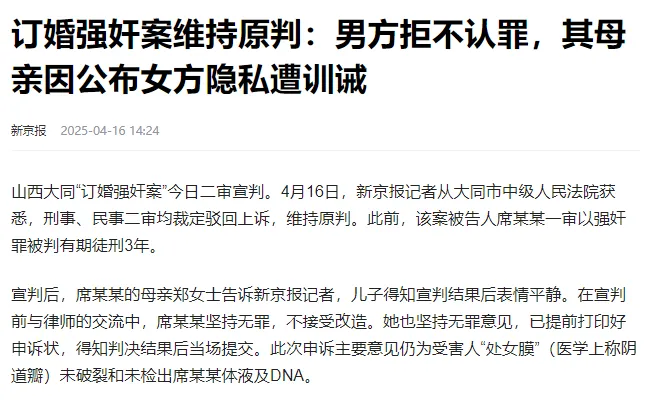
\includegraphics[width=13cm]{2025-04-17-001.png}
\end{figure}

此结果引发了巨大的舆论争议。

在法律上孰是孰非早就有无数人从无数角度说过了,此案“有巨大争议”而不是“一边倒”,那就说明是可这样判也可以不这样判,也就是确实可以这样判。

但此案拖延了2年多时间,全国各路人马已经对其进行了高强度显微镜级别的审视,结果仍然无法形成一边倒的决议,那就说明在法律层面是“可以”这样判的,并不是“绝对不能”这么判的。

但也绝不是“必须”这么判,否则此案就不需要拖延2年多,也不可能会引发那么大争议。

\zd{在法律的两可区域,判决倾向于哪边,那就是大案看政治了。}

虽然说此案两边的当事人都只是普通老百姓,但此事造成的影响力已经远远超过了普通舆论的范畴,对全国人民的婚恋情况都具有风向标的作用,属于典型的大案,甚至很多大案的重要性都没此案大。

这种案子怎么判,那已经不是基层法官能做主的了,肯定是层层请示的,而最终层层下达的结果就是维持原判,强奸罪成立,判3年有期徒刑。

一般来说只要引发了民意的剧烈抗议和负面反馈,很多市长乃至于更高级的官员都是瞬间被拿掉,因为我们政治的本质是为人民服务,只要判定为真实民意,合法性大过天,市长在这种力量面前和尘埃都差不多,大同市法院的几个法官没有那个通天的本领,不可能有人敢逆反民意去维护他们。

\zd{最后之所以维持原判,那是因为真实的民意就是要求维持原判,男方必须判强奸罪,舆论上喧嚣的那些都是假民意。}

民意之所以聚焦此案,真实的关注点并不是此案的法律纠纷细节,而是因为女方对彩礼的渴望。

只要男方同意房产加名,那此案就不是强奸案,别说最后拖延2年多,当初立案都立不起来,警察一开始就不愿意立案。

但如果男方不同意房产加名,那此案就是强奸案,最终也被判了强奸。

警方的调解持续到了最后一刻,男方也同意房产加名了,最后“差了几个小时”房本没有送到,到了法律规定的调解时限,随后警方正式立案,然后这事进入公诉阶段,就不是男女方还能改变的了。

男女方约定的彩礼确实只有18.8万,男方订婚时也只给了10万,但这半套房子的加名实质上就是彩礼,超高额变相彩礼,远远比那18.8万要多的多。

因为男方只给了10万就想行“夫妻之事”,低于女方预期的半套房子,所以女方觉得亏了,所以不加名那就报强奸,只要加名那就可以不报强奸。

\zd{某种意义上来说,这还真的是“违背妇女意志”,因为此案的女方意志很明确就是先拿到半套房子才能同房,这一点真实到没有任何人质疑。}

\zd{所以此案表面上是订婚案,实质上是彩礼案。}

而围观的群众,我指的是强烈反对大同一审判决,觉得男方冤屈的那批人,他们的真实诉求是什么?

\zd{\xhx{他们的真实诉求实质上是反对高彩礼,实质上是认为女方不应该收彩礼要房子,至于此案只是他们表达自己诉求的一个抓手而已。}}

\zd{你自己寻思下是不是这么回事。}

而支持者亦然,实质上就是借此想多要高彩礼,那些连法律条文都搞不清楚的人之所以反对或支持此案,然后争议巨大,实际上就是在争议这半套房子该不该给,或者说想不想给。

比大同订婚强奸案恶劣无数倍的真正强奸案那么多,你看有几个人关注?之所以那么多人关注这个案子实质上不就是因为此案的彩礼问题。

这个才叫真实民意。

\zd{找到了病根,才能开始治病,方向则是满足大多数人的利益。}

此案因为是彩礼案,又有男方女方的差别,所以有人故意把此案扭曲为男性和女性利益的对决,搞男女对立。

实质上这个世界上没有纯粹的男性和女性,只有那些无父无母无儿无女,兄弟姐妹亲戚朋友也没有,彻底孤寡一身的人,才可能是纯粹的男性或女性身份。

\zd{只要是正常中国人,身上都一定混合着多种身份,故意搞男女对立的,只有拿着海外钱故意使坏的各种组织、二极管,以及那些真正的坏人。}

就算是大同强奸案这件案子,负责拿出一辈子血汗钱出彩礼买房子,为了案情到处奔波的男方妈妈,那也是女的,她代表的是天下有儿子的所有女性,所以男方的身份并不是纯粹的男性。

所以满足大多数人利益的方向并不是男性女性,而非常明确的是降低彩礼,大同强奸案的判决结果必须使得社会彩礼会被降低。

\zd{那我问你,大同强奸案该怎么判,会使社会上的旁观男性愿意降低彩礼金额,而怎么判又会使这些男性愿意增加彩礼金额?}

\zd{你自己好好寻思寻思。}

在你寻思的过程中,我给你讲几个事实,来告诉你为什么这件事的影响力大上了天,最后的判决结果依然是强奸罪成立。

2025年的中央一号文件,是2025年全国各级政府工作的主要方向,而这份“天字号”文件上面白纸黑字写着要“治理高额彩礼”。

\begin{figure}[H]
    \centering
    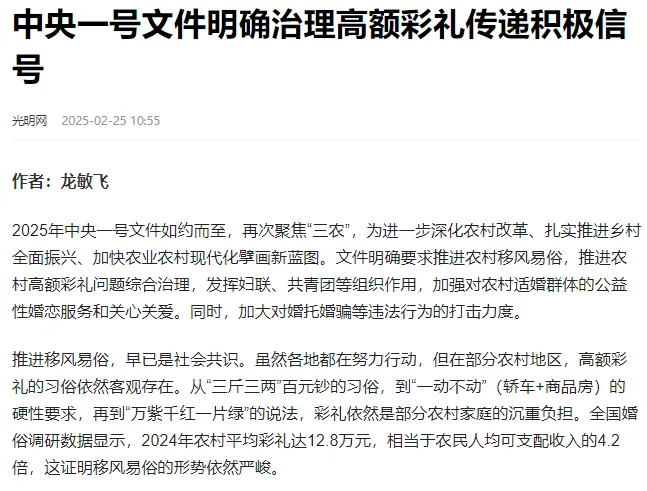
\includegraphics[width=13cm]{2025-04-17-002.png}
\end{figure}

但其实不止是2025年,2024年的中央一号文件也是要求治理高额彩礼,事实上从2019年开始中央一号文件就开始要求治理高额彩礼了,6年时间有5年的中央一号文件点名高额彩礼。

\begin{figure}[H]
    \centering
    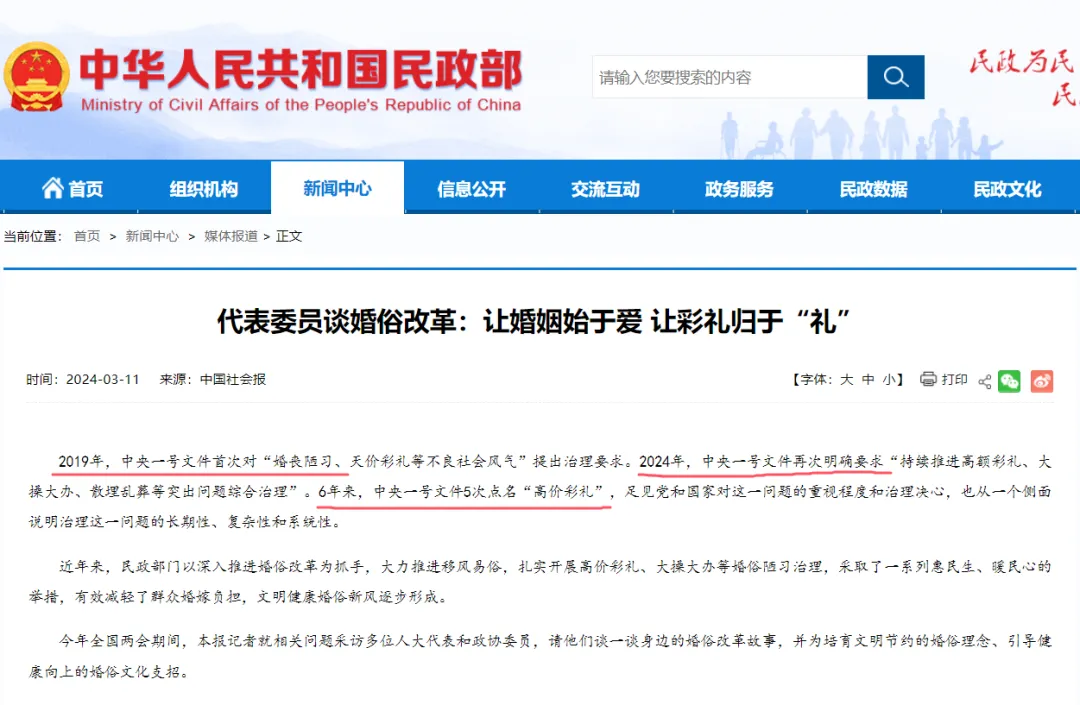
\includegraphics[width=13cm]{2025-04-17-003.png}
\end{figure}

\zd{你问我中央意志是什么,那很明显的中央意志就是要治理高额彩礼,把彩礼金额压下去。}

为贯彻落实这个中央意志,各级政府想出了且尝试了无数种办法。

国家电视台进行宣传,那是最起码的。

\begin{figure}[H]
    \centering
    
\includegraphics[width=13cm]{2025-04-17-004.png}
\end{figure}

在农村到处刷标语,搞宣传,那也是最起码的。

\begin{figure}[H]
    \centering
    
\includegraphics[width=13cm]{2025-04-17-005.png}
\end{figure}

派工作人员到处做宣讲工作,讲彩礼的危害,强调不要高彩礼,还是最起码的。

\begin{figure}[H]
    \centering
    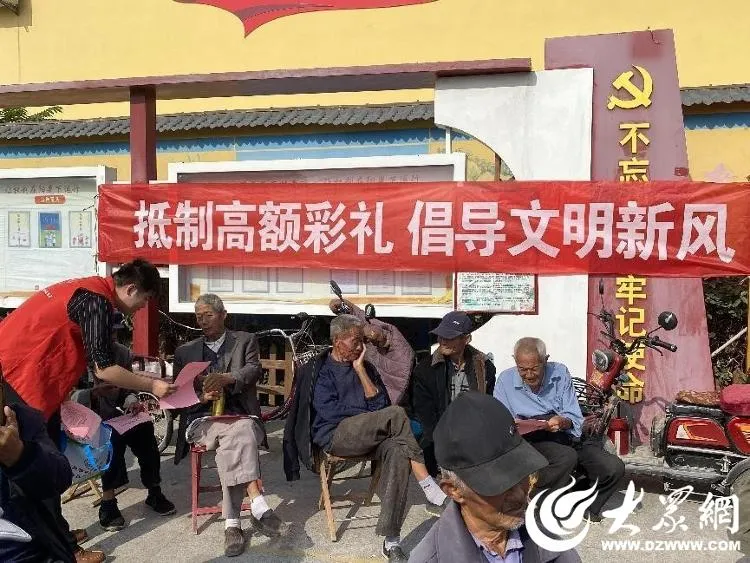
\includegraphics[width=13cm]{2025-04-17-006.png}
\end{figure}

最后还有被逼急的某地,宣布谁敢要高彩礼,就以贩卖人口罪论处,差点被人喷死。

\begin{figure}[H]
    \centering
    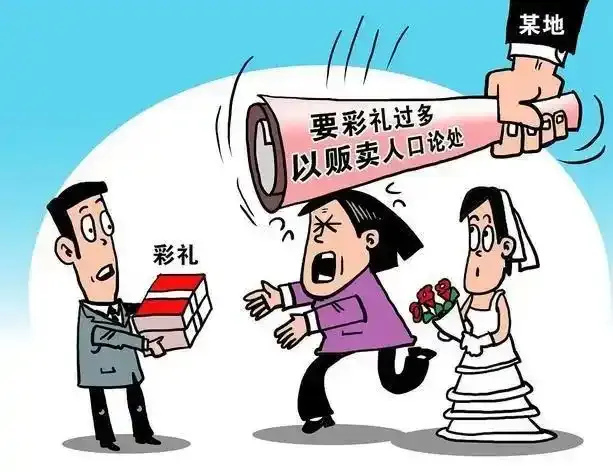
\includegraphics[width=13cm]{2025-04-17-007.png}
\end{figure}

所有手段尝试并努力的结果,是啥用都没有,全国彩礼金额一涨再涨,连年上涨,中央文件越强调要治理高额彩礼,那彩礼金额就越涨。

大量老百姓全家被彻底掏空,努力一辈子的血汗钱都拿出去甚至背负贷款,只为付个彩礼钱,一点办法都没有。

\begin{figure}[H]
    \centering
    
\includegraphics[width=13cm]{2025-04-17-008.png}
\end{figure}

因为高额彩礼的问题,因为那些彩礼钱已经高到了掏空男方一家的地步,而保障全无,全国酝酿出了无数的麻烦和冲突,也酿出了大量的惨案。

别人都给彩礼那自己也得给,否则儿子娶不到老婆,男方很难受。

而女方也很难受。

别人都收高彩礼,那自己也得收,不然就觉得自己“亏了”、“会被男方看不起”、“未来没保障”,很多本来很真挚的感情因为彩礼而闹翻了。

但这些彩礼绝大多数没有到女方手里。

对于家里有儿子的家庭,收到的彩礼转身就会变成儿子给其他女方家的彩礼,根本就不可能把这个钱给女方当嫁妆。

对于家里没有儿子的家庭,反正其他家的女儿出嫁也没有嫁妆,那我们为什么要给,爸妈帮你拿着多安全,打你账上万一被“坏男人”花光了下半辈子怎么办。

\zd{所以彩礼越高的地区嫁妆越少,彩礼最高的地区那嫁妆只有一床被子,而且无论女方家里有没有其他兄弟,统统都不会给嫁妆。}

因为这个是“习俗”,是“共识”,个人无法违逆社会共识,只能随波逐流,别人这么做自己也这么做。

\begin{figure}[H]
    \centering
    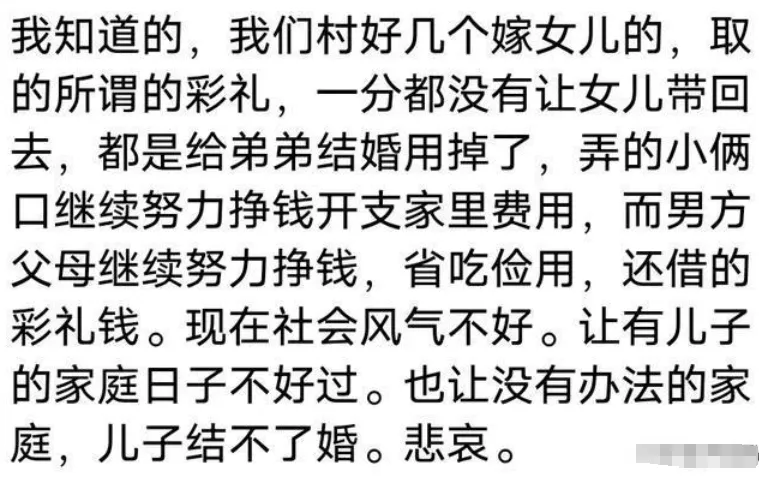
\includegraphics[width=13cm]{2025-04-17-009.png}
\end{figure}

所以女方从彩礼得利了吗?

如果女方是认认真真想和男方过一辈子的,那彩礼钱只要没有全部打回女方个人账户,女方就肯定是血亏,即便全部打回了女方个人账户,女方也只是不亏,谈不上得利。

能从这种事得利的只有那些从开始就没打算和男方过一辈子的,直接以婚姻名义骗钱的诈骗犯,钱到手直接离婚跑路,而且法律还没办法。

彩礼所具有的物化女性功能,到这里甚至都还没来得及考虑,光这种对和谐社会的严重破坏程度都必须要对其进行严厉治理了。

但治理的结果大家也看到了,手段尽出效果为零,关于中央一号文件要求治理高额彩礼的相关新闻下面是怎么评论的,大家应该都很清楚,清一色的是嘲笑,没人觉得光靠这个文件就能压制彩礼。

市场经济是无法违逆的,文件和宣传确实没有用,如果想结婚的适婚男性比想结婚的适婚女性多10%,而竞争方法只有彩礼一条路的时候,那彩礼金额就注定会涨到有10%的男性宁可不结婚也不愿意交这个彩礼,否则无法达成供需平衡。

在这可怕的市场力量面前,文件和宣传确实是没有用的,甚至法律都没有用。

最高法早就出规定了,明确禁止借婚姻索取财物,白纸黑字公告全国。

\begin{figure}[H]
    \centering
    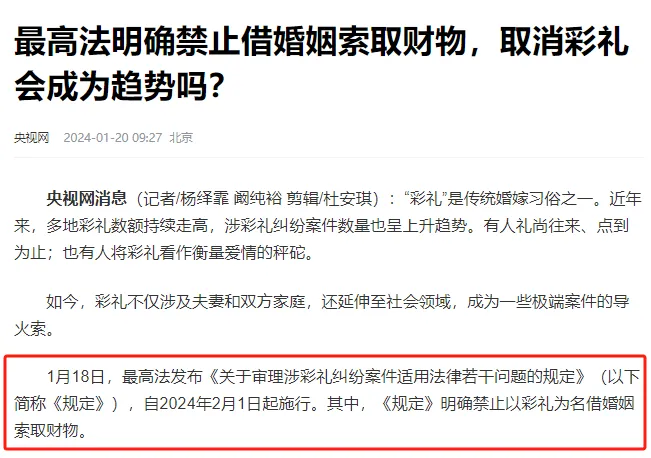
\includegraphics[width=13cm]{2025-04-17-010.png}
\end{figure}

但一点用没有,彩礼在民间不仅照收不误而且还持续上涨,这规定基本成了空气。

别管你怎么规定,民间永远有无数男性“自愿”给钱,直接的现金不同意给那就给房子,给黄金,给这个那个,只要男方自愿给,总有给的办法,你不可能拦得住。

\zd{因为有男性觉得花这个钱“有意义”,能“买到东西”,认为女方拿了钱必须跟他过一辈子,这批人压根不信法律会不保护自己给出去的彩礼,就非要疯狂给彩礼,以为万一女方反悔,只要报警上法庭肯定可以拿回自己给出去的彩礼。}

中央出文件没用,宣传没用,立法禁止也没用,好话已经说尽了,咋办?

那你说能咋办。

我不想这么做的,你们逼我的,我这也是为你们好。

\zd{现在你寻思好了没有,大同订婚强奸案,全国所有适婚男女都在关注的案件,怎么判会导致社会彩礼上升,怎么判会导致社会彩礼下降?}

都说大案看政治,没有啥政治能比中央一号文件更大了。

因为此案引发了全国的关注,因为此案成了全国婚恋的风向标,所以此案的判决结果必须要达到让围观的男性不敢付彩礼的目标,绝不能反过来。

在法律上有个基本常识,那就是:

\zd{\xhx{彩礼什么都不保证,也什么都买不到,彩礼给了就是白给。}}

\zd{\xhx{彩礼什么都不保证,也什么都买不到,彩礼给了就是白给。}}

\zd{\xhx{彩礼什么都不保证,也什么都买不到,彩礼给了就是白给。}}

重要的事情我强调三遍,别管民间觉得付了彩礼就能怎样怎样,但自新中国建国以来法律上就一直很明确,彩礼给了就是白给,如果严格按法律来说的话,那中国法律甚至压根就不承认彩礼这个东西。

给了就是赠予,白送,没有反悔一说,和是否结婚生孩子也一毛钱关系都没有,别人拿了彩礼下一秒就反悔走人且一分钱不退都是符合法律精神的。

不要出了事就找警察求助于法律,越是讲究法治精神,越是应该一分钱不退,因为法律上确实就是这么规定的,而且自建国以来就反对彩礼,你自己非要赠予那能怎么办。

但因为法律上的共识和民间的共识存在模糊地带,而且两种共识的差距太大,模糊地带太广,引发了诸多的矛盾和惨剧,在新的社会共识普遍形成之前,法律不得不进行了退让,于是出现了“以结婚为目的的赠予”这一法律解释,根据具体情况适当的退回给男方一部分彩礼。

如果严格执行法律,严格遵循中央一号文件治理高额彩礼的精神,那就不应该出现“以结婚为目的的赠予”这种说法,也应该一分钱不退给男方,只有一分钱不退才能最大程度的体现禁止彩礼的法治规定,才能最大程度的压制彩礼金额。

\zd{这么搞是为了缓解社会矛盾,是为了适应实际,是没办法里的折中办法,是社会共识过渡期里的过渡办法。}

很明显这种过渡期是比较难受的,既不符合民间共识也不符合法治共识,这个“适当返还”那是真的很难适当,自由裁量权太大,涉及金额太大。

所以尽快缩短这个过渡期,尽快形成新的社会共识,就成了国家需要完成的工作任务。

要形成新的社会共识只能靠宣传,而正的宣传之路既然走不通,那就只能反着走了,这条路其实不太好,必有损失,但确实没办法。

\zd{人教人教不会,事教人,那一教就会。}

不是喜欢给高彩礼么,不是越禁止就越要给高彩礼么?

给我找典型案例,全国曝光,吸引的注意力越多越好,力度要把控好,事不能太小但也不能太大,争取以最小的损失达成最大的教育成果。

这个做法和网上那些喊着要“请先生赴死”的口号,原理上是一样的。

大同订婚强奸案,2年前就有人喊着要判男方死刑,二审结果出来后还有人喊着要判男方死刑。

\begin{figure}[H]
    \centering
    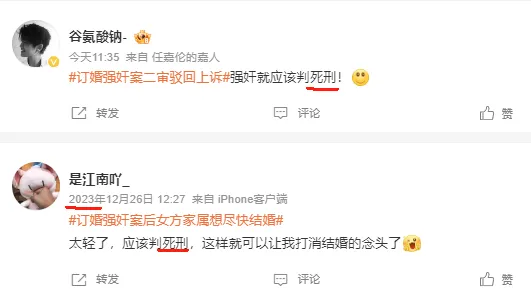
\includegraphics[width=13cm]{2025-04-17-011.png}
\end{figure}

这两个人不用猜,肯定是男性且为适婚男性然后讨厌高彩礼,希望判此案男方死刑的原因只有一个,那就是这种结果会最大程度的震慑敢付彩礼的人,会让社会彩礼大幅降低,从而让自己付彩礼的压力下降。

和其他适婚男性比,这两个人算是聪明人,知道怎么才能达成自己的真实诉求,就是手段太极端了,无冤无仇,人家法院才判3年,为了自己的利益希望此案的男方去死,有点过分了。

在大同订婚强奸案里,最终判男方三年有期徒刑,这实质上已经在法律范围内尽可能的倾向于男方了。

如果给彩礼等于白给,如果订婚不等于结婚,如果女方的意志确实是给了半套房才能上床,那男方的做法确实是实打实的“违反妇女意志”,这几点都确认清楚之后判刑没毛病,无非就是判多久的问题,虽然和民间共识矛盾很大。

而强奸罪的刑期是3~10年,真要是完全追求降低彩礼的宣传诉求,那也可以判10年,更吓人,男方更委屈,宣传效果更好。

\zd{如果仅考虑会增加还是减少社会彩礼金额这一个维度,那你觉得怎么判这个男方最合适?}

是无罪释放,还是判3年,还是判10年,亦或者按照网友的判决给个死刑?

最终的结果是3年,而且多次尝试想给个缓刑,这其实也有考虑新旧社会共识冲突,取折中之意了,同时虽然判决有倾向性,但也只是在法律两可范围内取倾向性,并没有为了达成教育宣传效果而偏离太远。

类似的典型案例还有重庆胖猫案,央视对胖猫案的定性让很多人极其愤怒,看不懂。

谭竹怎么能是无辜?胖猫怎么能是活该?

央视定性第一次被全国怒喷,你可以说是央视里有人水平差,感受不到民意。

但被喷完之后央视每隔一段时间就重新把此事给宣传一遍,越喷就越宣传。

当开始第三波宣传胖猫案定性的时候,脑子再迟钝的人都应该反应过来了,这不是水平差,是故意的,就是因为宣传效果好才反复拿出来宣传的。

这还是在宣传此事引发的民意有损自身威信的前提下,不理解只狂喷的人太多了,否则宣传的会更频繁。

\xhx{央视的宣传目的很简单,避免下一个胖猫再次出现,所以要反复宣传恋爱过程中给钱就是白给,胖猫就是榜样。}

\zd{给胖猫叫屈的人越多,那就说明宣传效果越好,同时也说明了宣传效果还没到位,需要再次宣传,一直宣传到这些人不给胖猫叫屈,觉得就是不应该这么无脑给钱为止。}

官方给胖猫叫屈,严惩谭竹,那只会导致更多的胖猫出现,等发现的时候人都沉江里了,再也不能复生。

这些年老有人说比萨斜塔,尤其是胖猫案话题下。。。

但实际上塔从来没斜过,塔的方向一直牢牢站在能降低社会彩礼的那个位置,胖猫给谭竹的恋爱赠予,实际上就是以婚姻为目的的赠予,实质上就是彩礼,绝不可鼓励和支持。

重要的事情重复三遍,恋爱结婚都可以,但\zd{给钱就是白给,给钱就是白给,给钱就是白给,}这就是官方想让你们达成的新社会共识。

\zd{给钱代表自愿赠与,钱买不到感情,买不到女人,买不到婚姻的保障,法律也不允许买得到,新中国自建国以来就不允许买得到,所以给钱必须是白给。}

而这条规定不止是中国有,所有现代文明国家都有,这不止是中国共识,是所有法治国家的一致共识。

不允许以彩礼多寡来获得婚恋竞争的优势,但婚恋竞争仍然在持续,那就只能从其他方面来入手了,所以和我们同文化的日韩男性早就开始把越来越多的钱投资在自己身上了,穿好衣服用好东西,打扮的好一点,甚至美容化妆,然后大量锻炼说话技术,给女性提供情绪价值,买房存款量力而为,不强求,避免自己压力过大成为蓬头垢面的赚钱机器。

这种做法会让男性年轻的时候拥有数量远超正常婚恋路线的异性数量,等老了对异性也没那么渴望了。

但很明显,这种做法会导致男性只谈恋爱不结婚,因为压根就没准备好结婚的资源,钱全砸自己身上以及谈恋爱去了,而事实上也是这样的,欧美日韩的结婚率都暴跌,年轻人全在谈恋爱。

对缓解男女数量矛盾来说,这个办法其实很有效,因为全谈恋爱,而不是一对一私有的话,那每个人拥有的异性数量都暴增,一辈子碰不到一个异性的人是极少数。

一个男性一辈子找3个女性,一个女性一辈子找3.3个男性,那就没有男女人数差距了,而且所有人都觉得自己挺那个的,没人觉得自己是光棍,恋爱的空档期那就独处,等年龄大一点荷尔蒙消退了就没找对象的欲望了,对独处也习惯了,慢慢就这样了,也不抱怨了。

对全社会来说优点很明显,缺点也很明显,那就是婚姻制度会解体,生育率也必然暴跌,欧美日韩的现状就是如此,目前的生育率都是用移民和私生子撑起来的。

没办法,甘蔗没有两头甜,不能既要又要,如果没有副作用那就没必要到迫于无奈的时候才会用。

但婚姻制度这东西,本身就是父系社会发明出来用来约束男性的,强行捆绑男性到固定家庭以便于提升幼儿的成活率,以便于提升国家的总人口,人类文明绝大多数时间都是没有婚姻制度的,进入农业社会且进入父系社会之后才慢慢发明出来,历史距今最多不超过5000年。

恩格斯当年写《家庭、私有制和国家的起源》的时候,就明确说过婚姻是因为私有制的诞生而诞生的,是一种压迫,所以要消灭婚姻。

封建社会是通过私有化女性来构建完成婚姻制度的,得到了远超母系社会的婴儿存活率,但恩格斯说的解放压迫,说的是男女所有人。

百年前的人接受不了,觉得太极端了,你现在觉得恩格斯是否为先知?

而构建在私有制下的婚姻制度,唯一的好处就是爆人口快,繁衍人口速度远超其他制度。

但近半个世纪以来,人口成了负担,全球没有任何一个国家想要更多的人口,欧美日韩想提振生育率也不是为了更多人口,而只是为了防止人口过快下降导致老龄化问题而已,最终目标还是想下降人口。

如果国家不需要很多很多的新增人口,那婚姻制度是真的没啥用。

因此如今的婚姻制度剥离了很多很多的私有制,剥离到几乎啥都没有了,婚姻几乎什么都不代表了,权力和义务皆无。

结了婚不代表女方就是男方的人了,也不代表男方就是女方的人了,不对双方具备任何的强制性,具备婚姻关系并不代表你有权力要求对方干嘛干嘛,对方想离就离,想走就走,想拒绝就拒绝,无论男女双方皆如此。

重要的事情说三遍。

\zd{婚姻什么都不保证,结婚证只能保证你可以平分婚后财产。}

\zd{婚姻什么都不保证,结婚证只能保证你可以平分婚后财产。}

\zd{婚姻什么都不保证,结婚证只能保证你可以平分婚后财产。}

中国的法律条文是这么写的,欧美日韩的法律条文也是这么写的,现代法治社会都是这么做的。

这好不好,不在今天的讨论范围之内,因为这是地球现状的客观事实,是大环境,你我都改变不了大环境。

而且根据恩格斯当年的理论,这一现状是必然的,是历史趋势,是人力无法改变的。

除非地球人口突然大减,否则没有恢复旧制度的可能性,因为旧制度唯一的好处就是爆人口快,其他全是缺点。

回到大同订婚强奸案,男方和女方是2023年1月30日在当地婚介所认识的,5月1日双方就订婚约了,同时给钱给房子。

很明显双方没有好好恋爱,女方愿意进入婚姻的主要动力也是那半套房,而不是男方这个人。

这样的婚姻即便能成,即便不因为强奸案闹掰,日后的婚姻生活也必定是一地鸡毛,想夫妻和睦幸福美满简直是做梦。

\zd{有钱确实是优势,但这个优势只存在于你没给钱之前。}

\zd{给完钱之后,那你还有啥优势,你还能继续按这种规模持续给钱吗?}

\zd{给那么多钱双方才能平等,那给完钱之后没钱了呢?}

不这么搞,也许女方会觉得夫妻是平等的,但这么一搞之后,只要会算数的女方,都会觉得不能再持续给钱的男方已经和自己不平等了,除非还能继续大规模给钱。

不能的话,那全家每天必然鸡飞狗跳,因为在这种算数下男方已经成了一个浑身缺点的纯劣势人,而婚姻又是自由的,毫无约束的,所以女方看不起男方想离婚,那是必然结果。

然后这么做的女方,因为耽误了最青春的年龄,又有婚姻经历,实际上是很难找到一个真心对自己的男性的,结局绝大多数都是一地鸡毛,双输。

要杜绝这种悲剧,那一开始就要杜绝为了钱而结婚这种事。

\zd{找一个爱自己人的伴侣,比找一个爱自己钱的伴侣,要重要的多。}

\zd{当你躺在急救室的时候,门外的伴侣在祈祷什么,取决于当初你自己找了一个什么样的伴侣。}

\xhx{男方是家庭赚钱的主力军,没钱确实没办法结婚,但男方要娶的女性,首先应该看重的是男方这个人,然后看重的应该是男方未来的钱,也就是婚后财产,这样形成的家庭才能稳固,男女方才能相亲相爱。}

\zd{\xhx{钱可以是男方的优势,但必须是持续有钱,可以持续提供这个优势,一次性给的钱必定会形成男方的劣势。}}

而大多数青年在适婚的年龄,手中的存款是约等于零的,大多数都是刚工作,只有未来的收入,所以结婚的彩礼实际上全是父母的存款。

家里有儿子的父母占一半,家里只有女儿但希望女儿过得好的又占了剩下的一半,还有部分是有女也有儿的,在剩下的零头里还有一些是女方自己希望能找到心仪伴侣好好过日子的。

所以降低彩礼金额确实是符合大多数人利益的,是会得到大多数人支持的,只有极少数骗婚的会反对。

以上这大部分人,对于大同订婚强奸案的判决结果的评价,方向都会是朝着降低社会彩礼金额而发力的,因为这是其利益所在。

无论男女,找到一个自己满意并且满意自己的伴侣,每天都打扮好自己,互相输出情绪价值,把钱当成生活的基础而不是主宰,一起和和美美过日子,多好。

\zd{所以大同订婚强奸案确实该大面积宣传,宣传的越多那新社会共识的形成就会越快,感情好的夫妻比例就会越大,社会才能越和谐。}

\zd{我不知道你是男是女,也不知道你的家庭情况和身份,那你觉得大同订婚强奸案如今的判决结果,是不是对你最有利的?}

\rule{.9\linewidth}{1pt}

\dianping{
    远方青木的这篇文章,重点关注的不是事件的是非曲直,而是判决对彩礼的影响,分析的角度比较新颖。
}

\end{document}

